\documentclass{article}
\usepackage[12pt]{extsizes}
\usepackage[T2A]{fontenc}
\usepackage[utf8]{inputenc}
\usepackage[english, russian]{babel}

\usepackage{amssymb}
\usepackage{amsfonts}
\usepackage{amsmath}
\usepackage{enumitem}
\usepackage{graphics}
\usepackage{graphicx}

\usepackage{lipsum}

\newcommand{\definebox}[3]{%
	\newcounter{#1}
	\newenvironment{#1}[1][]{%
		\stepcounter{#1}%
		\mdfsetup{%
			frametitle={%
				\tikz[baseline=(current bounding box.east),outer sep=0pt]
				\node[anchor=east,rectangle,fill=white]
				{\strut #2~\csname the#1\endcsname\ifstrempty{##1}{}{##1}};}}%
		\mdfsetup{innertopmargin=1pt,linecolor=#3,%
			linewidth=3pt,topline=true,
			frametitleaboveskip=\dimexpr-\ht\strutbox\relax,}%
		\begin{mdframed}[]\relax%
		}{\end{mdframed}}%
}

\definebox{definition}{Определение}{blue!24}
\definebox{task}{Задача}{orange!24}

\usepackage{geometry} % Меняем поля страницы
\geometry{left=1cm}% левое поле
\geometry{right=1cm}% правое поле
\geometry{top=1.5cm}% верхнее поле
\geometry{bottom=1cm}% нижнее поле


\usepackage{fancyhdr} % Headers and footers
\pagestyle{fancy} % All pages have headers and footers
\fancyhead{} % Blank out the default header
\fancyfoot{} % Blank out the default footer
\fancyhead[L]{ЦРОД $\bullet$ Математика}
\fancyhead[C]{\textit{Геометрия}}
\fancyhead[R]{ЛФМШ 2023}% Custom header text


%----------------------------------------------------------------------------------------

%\begin{document}\normalsize
\begin{document}\large
	
	\begin{center}
		\textbf{Теорема Паскаля}
	\end{center}
	
	\textbf{Теорема Паскаля:} Точки пересечения противоположных сторон вписанного шестиугольника лежат на одной прямой.
	
	\textbf{Обратная теорема Паскаля:} Если пять вершин шестиугольника лежат на одной окружности, и точки пересечения противоположных сторон лежат на одной прямой, то и шестая точка тоже лежит на этой окружности.
	
	\textbf{Как использовать?} Пронумеруем вершины ломанной от 1 до 6. Пусть 
	$12 \cap 45 = 7$; $23 \cap 56 = 8$; $34 \cap 61 = 9$. Тогда точки 7, 8, 9 лежат на одной прямой.
	
	При этом можно «склеивать» точки. Например, если склеить точки 1 и 2, то прямая 12
	превратится в касательную к окружности.
	Примеры склеивания точек можно посмотреть на обратной стороне листа.
	
	\begin{enumerate}[label*=\protect\fbox{\arabic{enumi}}]
		
		\item Доказать, что во вписанном четырехугольнике точки пересечения противополож- ных сторон и точки пересечения касательных в противоположных вершинах лежат на одной прямой.
		
		\item Даны треугольник $ABC$ и некоторая точка $T$. Пусть $P$ и $Q$ — основания перпендикуляров, опущенных из точки $T$ на прямые $AB$ и $AC$ соответственно, a $R$ и $S$ — основания перпендикуляров, опущенных из точки $A$ на прямые $TC$ и $TB$ соответственно. Докажите, что точка пересечения прямых $PR$ и $QS$ лежит на прямой $BC$.
		
		\item Внутри треугольника $ABC$ выбрана точка $M$. Прямые $AM, BM, CM$ пересекают описанную окружность треугольника $ABC$ в точках $A', B', C'$ соответственно. Докажите, что главные диагонали шестиугольника, образованного пересечением треугольников $ABC$ и $A'B'C'$, пересекаются в точке $M$.
		
		\item Окружность, проходящая через вершины $A$ и $D$ основания трапеции $ABCD$, пересекает боковые стороны $AB, CD$ в точках $P, Q$, а диагонали — в точках $E, F$. Докажите, что прямые $BC, PQ, EF$ пересекаются в одной точке.
		
		\item Дан прямоугольник $ABCD$ и точка $P$. Прямые, проходящие через $A$ и $B$ и перпендикулярные, соответственно, $PC$ и $PD$, пересекаются в точке $Q$. Докажите, что $PQ \perp AB$.
		
		\item Точка $M$ лежит на описанной окружности треугольника $ABC$; $R$ — произвольная точка. Прямые $AR, BR, CR$ пересекают описанную окружность в точках $A_1, B_1, C_1$. Докажите, что точки пересечения прямых $MA_1$ и $BC$, $MB_1$ и $CA$, $MC_1$ и $AB$ лежат на одной прямой, проходящей через точку $R$.
		
		\item Пусть $A'$ — точка, диаметрально противоположная точке $A$ в описанной окружности треугольника $ABC$ с центром $O$. Касательная к описанной окружности в точке $A'$ пересекает прямую $BC$ в точке $X$. Прямая $OX$ пересекает стороны $AB$ и $AC$ в точках $M$ и $N$. Докажите, что $OM = ON$.
		
		\item Равносторонний треугольник $ABC$ вписан в окружность $\Omega$ и описан вокруг окружности $\omega$. На сторонах $AC$ и $AB$ выбраны точки $P$ и $Q$ соответственно так, что отрезок $PQ$ проходит через центр треугольника $ABC$. Окружности $\Gamma_b$ и $\Gamma_c$ построены на отрезках $BP$ и $CQ$ как на диаметрах. Докажите, что окружности $\Gamma_b$ и $\Gamma_c$ пересекаются в двух точках, одна из которых лежит на $\Omega$, а другая --- на $\omega$.
		
		\item Точка $M$ — середина гипотенузы $AC$ прямоугольного треугольника $ABC$. Точки $D$ и $E$ на отрезках $AM$ и $AB$ соответственно выбраны так, что $BC \parallel DE$. Окружность $\omega$, описанная около треугольника $ABC$, пересекает описанную окружность треугольника $CDE$ в точках $C$ и $F$, а прямую $DE$ в точках $X$ и $Y$. Касательная к окружности $\omega$ в точке $B$ пересекает луч $FC$ в точке $Z$. Докажите, что описанные окружности треугольников $XMY$ и $BFZ$ касаются.
		
	\end{enumerate} 
	
	\begin{figure}[h]
		\center{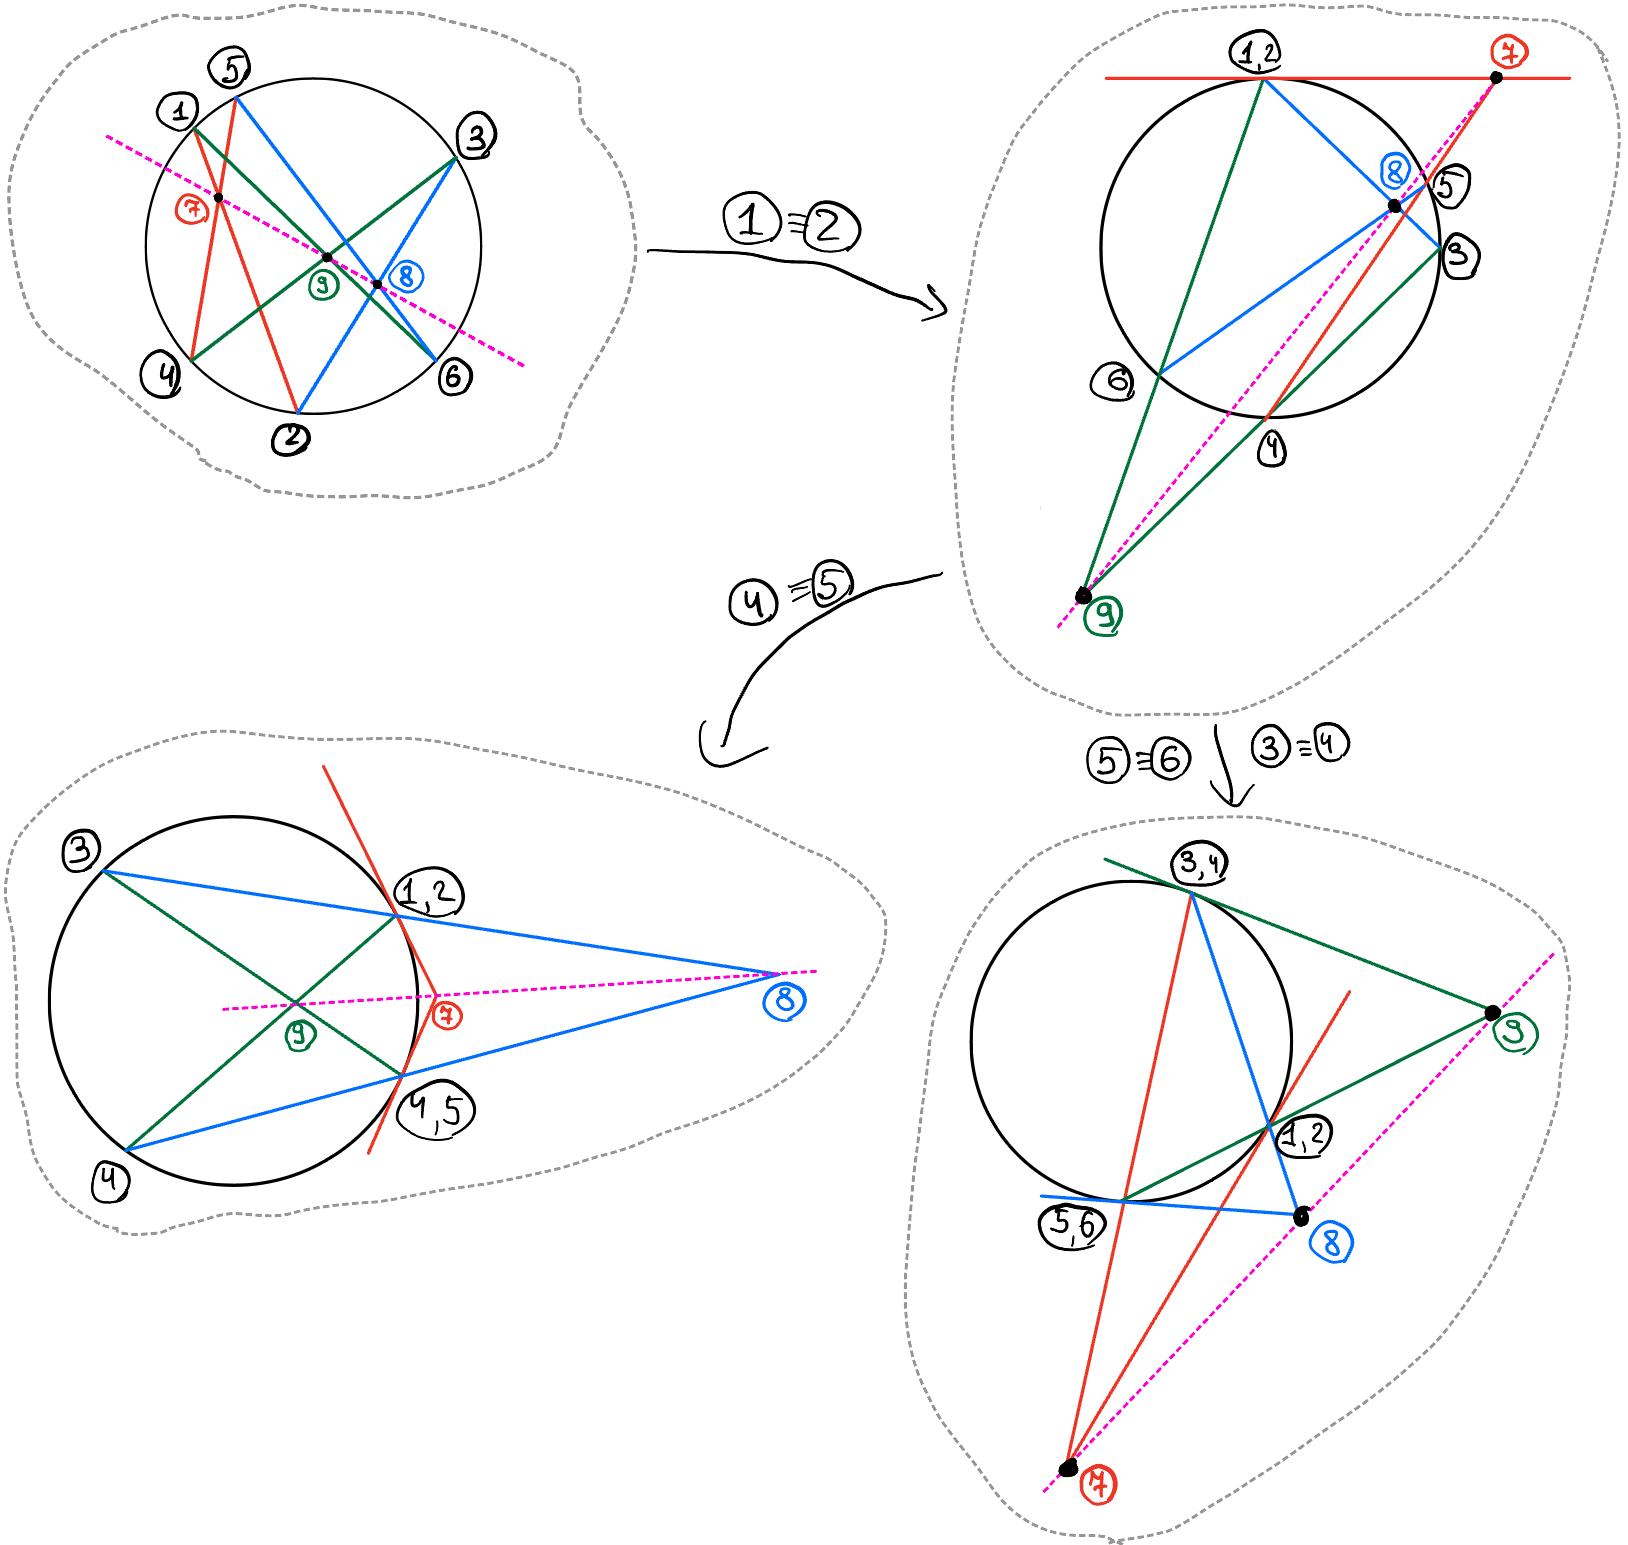
\includegraphics[width=0.875\linewidth]{img1.png}}
		\caption{Примеры склейки точек}
	\end{figure}
\end{document}